\chapter{Teoretisk Grunnlag}
\label{chap:co_theory}

\section{Betingelseskvalifikasjoner}
\label{sec:constraint_qualifications}
For å sikre at optimalitetsbetingelsene er gyldige og at vi kan finne Lagrange-multiplikatorer, trenger vi visse betingelser kjent som "constraint qualifications".

\section[Slaters betingelse]{\gls{slater-condition}}

\begin{definition}[breakable]{Slaters betingelse}{slater_condition}
	For et konvekst problem med ulikhetsbetingelser
	\[
		c_i(x) \le 0,\quad i=1,2,\dots,m,
	\]
	er Slaters betingelse oppfylt dersom det finnes et \(x\) slik at
	\[
		c_i(x) < 0 \quad \text{for alle } i.
	\]
\end{definition}

\begin{remark}{Intuisjon}{}
	Denne betingelsen garanterer at det tillatte området har et ikke-tomt indre.

	Med andre ord: Betingelsene er ikke alle \enquote{stramme} i hvert punkt, noe som sikrer sterk dualitet og eksistens av Lagrange-multiplikatorer.
\end{remark}

\section{Lineær Uavhengighetsbetingelse (LICQ)}
\label{sec:LICQ}

Et ikke-lineært optimeringsproblem kan skrives på følgende måte\cite[Kapittel~12]{NocedalWright2006}:
\begin{mini*}
	{x \in \mathbb{R}^n}{f(x)}{}{}
	\addConstraint{c_i(x)}{= 0,\quad}{ i \in \mathcal{E}}
	\addConstraint{c_j(x)}{\leq 0,\quad}{ j \in \mathcal{I}}
\end{mini*}

Hvor \(f : \mathbb{R}^n \to \mathbb{R}\) er den vanlige objektfunksjonen vår, men hvor \(c_i(x)\), \(c_j(x)\) representerer henholdsvis likhets- og ulikhetsbetingelser (kravene til løsningsrommet vårt \(\Omega\)).

\subsection{Definisjon av LICQ}

\begin{definition}{Linear Independence Constraint Qualification (LICQ)}{licq}
	La $x^*$ være et \emph{feasibelt} punkt. Definer mengden av aktive betingelser
	\[
		\mathcal{A}(x^*) \;=\; \{\; i \in \mathcal{E} \cup \mathcal{I} \;\mid\; c_i(x^*) = 0 \}.
	\]
	LICQ er oppfylt ved $x^*$ hvis gradientene til de aktive betingelsene
	\[
		\{\nabla c_i(x^*) :\, i \in \mathcal{A}(x^*)\}
	\]
	er lineært uavhengige i $\mathbb{R}^n$. Formelt betyr dette:
	\[
		\sum_{i \,\in\, \mathcal{A}(x^*)} \lambda_i \,\nabla c_i(x^*) \;=\; 0
		\quad \Longrightarrow \quad
		\lambda_i = 0 \;\;\text{for alle}\; i \in \mathcal{A}(x^*).
	\]
\end{definition}

\begin{remark}{Betydning av LICQ}{}
	LICQ sikrer at standard Karush--Kuhn--Tucker-(KKT)-teori er anvendelig, blant annet fordi:
	\begin{itemize}
		\item Eventuelle Lagrange-multiplikatorkoordinater (for de aktive betingelsene) er veldefinerte
		\item Disse multiplikatorene er ofte unike
		\item KKT-betingelsene blir nødvendige optimalitetsbetingelser
	\end{itemize}
\end{remark}

\subsection{Rollen til LICQ i KKT-teori}

Følgende punkter fremhever hvorfor LICQ er sentralt:
\begin{enumerate}
	\item \textbf{Eksistens av Lagrange-multiplierne:} Hvis \(x^*\) er et lokalt minimum og LICQ gjelder ved \(x^*\), eksisterer en unik vektor \(\lambda^*\) av multiplikatorer for de aktive betingelsene slik at KKT-betingelsene
	      \[
		      \nabla f(x^*) \;=\; \sum_{i \,\in\, \mathcal{A}(x^*)}\!\lambda_i^*\,\nabla c_i(x^*),\quad
		      \lambda_j^* \,\ge\,0 \text{ for aktive ulikheter},
	      \]
	      samt komplementaritetsbetingelser, blir oppfylt.
	\item \textbf{Lokal regularitet:} Dersom LICQ holder, har Jakobi-matrisen for de aktive betingelsene full rang.
	      Dette sikrer at gradientene til de aktive betingelsene er lineært uavhengige, noe som er nødvendig for å kunne bruke KKT-betingelsene.
	\item \textbf{Unikhet av multiplikatorer:} Hvis LICQ er oppfylt, er multiplikatorene entydige. Dette betyr at det ikke finnes flere løsninger for multiplikatorene som tilfredsstiller KKT-betingelsene.
\end{enumerate}
Hvis LICQ ikke holder, kan det oppstå problemer med å finne Lagrange-multiplikatorene, og KKT-betingelsene kan bli ugyldige eller gi flere løsninger.
\begin{example}{LICQ med flere ulikhetsbetingelser}{}
	La oss se på følgende optimeringsproblem med diverse ulikhetsbetingelser:
	\begin{mini*}
		{x,y}{(x-1)^2 + (y+2)^2}{}{}
		\addConstraint{c_1(x,y) &= -x}{\leq 0}{}
		\addConstraint{c_2(x,y) &= x-2-y}{\leq 0}{}
		\addConstraint{c_3(x,y) &= 1-(x-1)^2-y^2}{\leq 0}{}
	\end{mini*}

	Ved punkt \(P\) hvor alle tre betingelser møtes, har vi følgende gradienter:
	\begin{align*}
		\nabla c_1(x,y) & = (-1,0),        \\
		\nabla c_2(x,y) & = (1,-1),        \\
		\nabla c_3(x,y) & = (-2(x-1),-2y).
	\end{align*}

	% Taken from: TMA4180 - Optimization 1 - NTNU 
% Exam Autumn 2024 - Problem 2

\documentclass[tikz,border=5pt]{standalone}
\usepackage{tikz}

\begin{document}

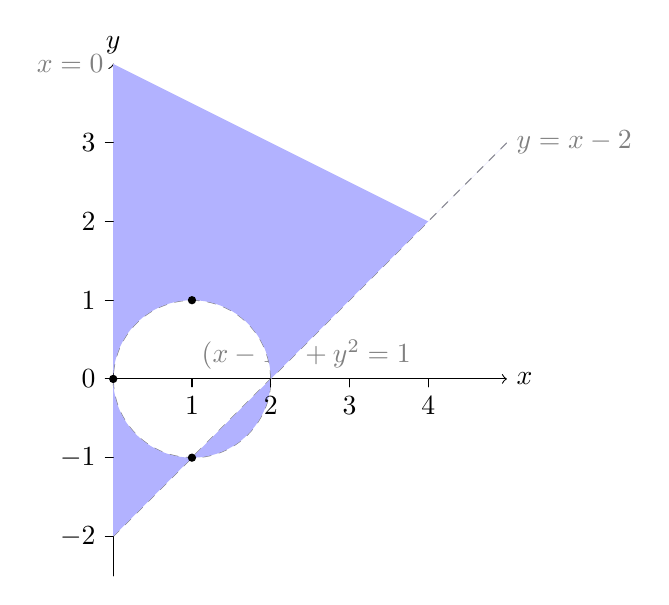
\begin{tikzpicture}[scale=1, line cap=round, line join=round]

  \draw[->] (-0.1,0) -- (5,0) node[right] {\(x\)};
  \draw[->] (0,-2.5) -- (0,4) node[above] {\(y\)};
  
  % Feasible region: outside the circle, with x ≥ 0 and y ≥ x − 2
  \draw[dashed, color=gray] (0,-2) -- (5,3) node[right]{\(y=x-2\)};
  \draw[dashed, color=gray] (0,-2) -- (0,4) node[left]{\(x=0\)};
  \draw[dashed, color=gray] (1,0) circle (1) node[above right]{\((x-1)^2+y^2=1\)};
  \node at (1,2) {\(\Omega\)};
  \fill[blue!30, even odd rule] 
    (0,-2) -- (5,3) -- (4,2) -- (0,4) -- cycle
    (1,0) circle (1);
    
  \foreach \x in {1,2,3,4}{
    \draw (\x,0) -- (\x,-0.1) node[below] {\(\x\)};
  }

  \foreach \y in {-2,-1,0,1,2,3}{
    \draw (0,\y) -- (-0.1,\y) node[left] {\(\y\)};
  }

  \fill (1,1)   circle(1.5pt);
  \fill (0,0)   circle(1.5pt);
  \fill (1,-1) circle(1.5pt);



\end{tikzpicture}

\end{document}


	Ved punkt \(P\) hvor alle tre betingelser møtes, kan vi se at gradientene peker i forskjellige retninger og er lineært uavhengige. Derfor er LICQ oppfylt ved dette punktet.

	Dette er viktig for å kunne bruke KKT-betingelsene til å finne den optimale løsningen.

\end{example}


\begin{remark}{LICQ -- Kort Fortalt}
	LICQ består av to nøkkelelementer:
	\paragraph{Aktive betingelser} En betingelse er aktiv hvis:
	\[ \begin{cases}
			c_i(\symbf{x}) = 0 & \text{for likhetsbetingelser}         \\
			c_j(\symbf{x}) = 0 & \text{for aktive ulikhetsbetingelser}
		\end{cases} \]
	\paragraph{Lineær uavhengighet} Gradientene \(\{\nabla c_k(\symbf{x}^\star)\}\) til de aktive betingelsene må være lineært uavhengige, altså:
	\[
		\sum_k \alpha_k \nabla c_k(\symbf{x}^\star) = 0 \implies \alpha_k = 0 \text{ for alle } k
	\]
\end{remark}

\subsection{Oppsummering}

Lineær Uavhengighetsbetingelse (LICQ) er en kjernenødvendighet for mange algoritmer og analytiske metoder innen ikke-lineær optimering. Den sikrer at de aktive betingelsene ved et punkt \(x^*\) er ``pent'' ordnet, i den forstand at ingen av gradientene er lineært avhengige. Når LICQ er gyldig, kan man utlede KKT-betingelsene og ofte fastslå entydige multiplikatorer. Som eksempel viser vi at betingelser som er multiple av hverandre (redundante) fører til brudd på LICQ og kan komplisere både teori og numeriske metoder.
